\documentclass[egregdoesnotlikesansseriftitles]{scrartcl}

\usepackage[T1]{fontenc}
\usepackage[utf8]{inputenc}

\usepackage{amsmath}
\usepackage{amssymb}
\usepackage{authblk}
   \renewcommand\Affilfont{\small}
\usepackage{dcolumn}
   \newcolumntype{d}[1]{D{.}{.}{#1}}
\usepackage{float}
\usepackage{graphicx}
\usepackage[hidelinks]{hyperref}
   \urlstyle{rm}
\usepackage[authoryear]{natbib}
\usepackage{url}

\setcitestyle{aysep={}}

\deffootnote{1.5em}{1em}{\makebox[1.5em][l]{\thefootnotemark}}
   \setlength{\skip\footins}{1.5em}
   \setlength{\footnotesep}{1em}

\title{Equal Deeds, Different Needs}
\subtitle{Need, Accountability, and Resource Availability in Third-Party Distribution Decisions}

\author[1]{Alexander Max Bauer}
\author[2]{Jan Romann}

\affil[1]{ Department of Philosophy, University of Oldenburg,

Corresponding Author, E-Mail: \href{mailto:alexander.max.bauer@uni-oldenburg.de}{alexander.max.bauer@uni-oldenburg.de}}
\affil[2]{ SOCIUM Research Center on Inequality and Social Policy, University of Bremen}

\date{\small Forthcoming in \textit{Oxford Studies in Experimental Philosophy}}

\begin{document}
\maketitle

\vspace{\fill}
\noindent\textbf{Abstract:} In a vignette study with a quota sample of the German population ($n=400$), subjects had to redistribute a good between two hypothetical persons who contributed equally to the available amount but differed in quantity needed and the reason for their neediness.
Within subjects, it was tested for the effects of need, accountability, and resource availability.
Between subjects, kinds of needs were varied: Persons needed the good to survive, to live a decent life, to participate in society, or to be autonomous.
Despite equal productivity, the mean share allocated to the needier person was significantly higher than an equal share.
However, this share turned out significantly smaller when the needier person was accountable for needing more.
Nonetheless, even if accountable, the needier person still got a share larger than their contribution.
When there was a surplus of resources, the needier person got a higher share than when resources were scarce.\\[2ex]

\noindent\textbf{Keywords:} Accountability, Distributive Justice, Equality, Equity, Need, Responsibility, Vignette Study\\[0.5ex]


\newpage
\section{Introduction}\label{sec:introduction}
Recently, the eyes of the world have turned to Russia and Ukraine.
And to the global oil and gas market.
In the wake of the war, prices have surged, and joint European action has been proclaimed, with Commission President Ursula von der Leyen stating that ``[w]e must become independent from Russian oil, coal and gas.
We simply cannot rely on a supplier who explicitly threatens us. 
We need to act now to mitigate the impact of rising energy prices, diversify our gas supply for next winter and accelerate the clean energy transition'' \citep[par. 3]{european_repowereu_2022}.
With or without secured supplies, the next winter is coming.
And some people suddenly find themselves wondering: ``What would I do if I couldn't afford heating during winter?''

In the vignette study presented below, we look at two hypothetical persons, both short on money and in need of heating material.
In this situation, they get the opportunity to chop their own firewood.
Both manage to chop an equal amount of wood.
Our subjects' task, then, is to redistribute this wood among both persons in a way they deem to be most just.
They can give each person exactly what they have chopped, resulting in an equal share.
But: While both persons have chopped equally much, there are factors present that might lead subjects to distribute the wood unequally, nevertheless.
For example, both persons can differ in their kinds of needs (i.e., they can need the firewood for different purposes), which may seem to be differently important: Should a person who needs the wood to survive get more than a person who needs the wood to make art in their studio?
And if one person needs more than the other, should it make a difference whether or not this is due to self-inflicted health issues resulting from ignoring a doctor's warning to stop smoking?

Hence, we investigate whether subjects' ideas of justice, reflected in the hypothetical distribution decisions they made as impartial spectators, take into account factors like the kinds of needs or the accountability of a person, amongst others.
In doing so, we contribute to the numerous empirical studies on laypeople's distributive preferences that have been conducted in recent years (see, e.\,g., \citealt{bauer_philosophie_2019,bauer_empirical_2020} for perspectives on the interdependencies of such empirical endeavours and ethical theories).
Those preferences have been shown to be pluralistic; besides equality and equity, \textit{need} is regarded as an essential principle (see, e.\,g., \citealt{konow_fair_2001, konow_which_2003}, \citealt{weis_needs_2017}, \citealt{bauer_winter_2023}, also see \citealt{miller_needs-based_2020}) that is sometimes balanced against accountability (see, e.\,g., \citealt{konow_fair_2001}, \citealt{schwettmann_trading_2009}, \citealt{bauer_need_2022}).

We contribute to this literature by testing for the effects of need, accountability, and resource availability on third-party distribution decisions.
Subjects distributed a good among two fictional individuals who contributed equally to the amount available but needed different quantities of the good.
This was done with a quota sample of the German population, building upon prior work by \cite{bauer_need_2022}.
Thus, as a follow-up study, large parts of our design are fairly close to the original work.
Between subjects, we varied the kinds of experienced needs: The fictional persons either needed firewood to survive, live a decent life, participate in society, or be autonomous.
Within subjects, we further varied whether they had chopped more or fewer logs of wood than they needed themselves (a within-subjects variation already found in \citealt{bauer_need_2022}, albeit in a less systematic way) and whether or not one person was accountable for needing more wood than the other person (a variation that was originally done between subjects in \citealt{bauer_need_2022}).
Subjects had to redistribute the firewood in 20 different cases.
In the original study, the cases varied both the persons' needs and productivity.
We kept productivity equal and constant in order to alter the need as well as the resource availability in a more systematic manner.

Implementing the four different kinds of needs is a novel feature of our study.
Also, compared to \cite{bauer_need_2022}, we doubled both the sample size (from $n=200$ to $n=400$) as well as the number of distribution decisions each subject makes (from 10 to 20).
Concurrently, we changed the parametrization of all cases instead of simply adopting some from \cite{bauer_need_2022}.
Our new parametrization is designed to systematically vary the \textit{need share} of the first person (``Person A'') and introduces the two \textit{supply scenarios} as a novelty compared to \cite{bauer_need_2022}.
With these changes, we hope to get more fine-tuned data on these factors.

We find that there are no significant differences in distributive decision-making regarding the four types of needs (this might be because we have not made the four kinds of needs successfully salient; an effect has later been found in \citealt{bauer_winter_2023}).
Despite this, we found that subjects distribute unequally favouring the needier person across all four treatments.
The within-subjects analysis revealed that this is influenced both by accountability and resource availability.
The mean allocated to the needier person is significantly lower when the person is accountable for their greater need.
However, even when accountable, the needier person gets a share that still exceeds their initial contribution.
In general, the needier person gets an even higher share when there is a surplus of resources than when resources are scarce.
Hence, despite changes in the design of the follow-up study, key aspects of \citealt{bauer_need_2022} were successfully replicated.

The remainder of this brief chapter is organized as follows:
Section \ref{sec:literature} very shortly introduces the study's background.
Section \ref{sec:design} then describes the study's design.
The results of our analysis are presented thereafter in Section \ref{sec:results}.
Finally, Section \ref{sec:conclusion} concludes.


\section{Background}\label{sec:literature}
When talking about need, we mean needs that are not purely instrumental but \textit{fundamental}, \textit{categorical}, or \textit{basic} instead.
Such needs are distinguished from mere wants, wishes, or desires and bear normative force.
This might be the case, for example, when they are ``necessary, indispensable, or inescapable, at least with respect to some important goals'' (\citealt[par. 37)]{brock_needs_2019}.

Over time, the philosophical literature has proposed various lists of such needs, giving accounts of what specifically is deemed a need bearing normative force (e.g., \citealt{doyal_theory_1991}, \citealt{braybrooke_meeting_1987}, \citealt{nussbaum_aristotelian_1990}).
Some oppose such lists, though.
\citeauthor{hamilton_political_2003} (2003, p. 12), for example, states that ``they are \textit{meta}-political naturalisations of historically contingent human needs and ends because they entrench a single moment in a dynamic process'' and thus fail to grasp the true nature of needs.
As an alternative to such lists, he proposes a categorization of needs using a triptych of classes, namely \textit{vital needs}, \textit{social needs}, and \textit{agency needs}.

This, of course, is but the tip of the iceberg of the debate surrounding the concept of need.
And there is little to no consensus as to the extent of needs (i.e., what does count as need and what does not) and the question of how to categorize or order them.
Hence, we made a selection and chose four different kinds of needs that the literature often identifies as morally relevant: needs for mere survival, needs for a decent life, needs for social belonging, and needs for autonomy.\footnote{\cite{bauer_sated_2018,bauer_sated_2022} already hinted at the importance of differentiating kinds of needs both for the measurement of need-based distributive justice, which is his main focal point, as well as for empirical research on need-based distributive justice.}
Survival needs might be the hottest candidate for consensus among need theorists.
As far as we know, they all include such needs in their conceptions (to name but two examples, see \citealt{wiggins_needs_1987} and \citealt{daniels_just_1985}).
Next, \textit{decency} is often identified as important for needs.
Prominently, \citeauthor{miller_human_2007} (2007, p. 3) argues that what he calls ``basic needs'' are ``conditions for a decent human life in any society'' (see also \citealt{miller_principles_1999}).
Since humans ``are social as well as biological creatures'', they ``can be harmed by being denied the conditions of social existence'' \cite[p. 3]{miller_human_2007}.
Hence, we included needs for social belonging.
Lastly, as \citet{doyal_theory_1984,doyal_theory_1991} point out, a person's actions must not be imposed on them, they need autonomy (see also \citealt{hamilton_political_2003}, \citealt{brock_needs_2005}, \citealt{siebel_need-based_2020}).

Obviously, there is a rich philosophical debate not only regarding (kinds of) needs in general but also regarding the concepts of survival, decency, belonging, and autonomy.
This study, however, uses simplified interpretations of the four kinds of needs (see Section \ref{sec:design}) to uphold an uncluttered design and not overwhelm subjects.
Future studies should broaden the picture by taking into account different readings and aspects of those concepts.

When speaking of accountability, we have Konow's principle of accountability in mind.
This principle ``calls for allocations to be in proportion to volitional contributions'' (\citealt{konow_fair_2001}, p. 138) and demands that ``individuals are only held accountable for factors they may reasonably control'' (\citealt{konow_fair_2001}, p. 142).
In the context of distributive justice, one might also think of \textit{luck egalitarianism}, which argues that one being worse off than others can only be justified if they are accountable for being so.
The effects of \textit{brute luck} should therefore be compensated, while those resulting from \textit{option luck} do not qualify for compensation.

While there is no empirical literature known to us that distinguishes between kinds of needs as we understand and categorize them, several studies are concerned with the interplay of need and accountability.
A variety of studies found an influence of need moderated by accountability in different experimental settings and a wide variety of contexts (see \citealt{bauer_need_2022} for an overview).


\section{Study Design}\label{sec:design}
We adopted a vignette from \cite{bauer_need_2022} that introduces two hypothetical persons, henceforth \textit{Person A} and \textit{Person B}.
As both need firewood, the community they live in allows them to cut timber in the community forest.
Subjects had the task to redistribute the total amount of wood chopped among the two in a way they deemed as just as possible (vignettes and instructions can be found in Appendix \ref{sec:app_instructions}).
For the distribution tasks, subjects were given 20 different \textit{cases} in which we presented Persons A and B as having different quantities of need.
Their productivity was the same in all cases: Every time Persons A and B chopped an equal amount of 500 logs each.
Thus the subjects had 1,000 logs in total to redistribute in every case.

The 20 cases were split into two \textit{accountability frames} with 10 cases each.
\cite{bauer_need_2022} have already shown that this manipulation works between subjects; we adopt it as a within-subject variation.
In the \textit{high accountability frame}, Person A has a metabolic disease since they smoked heavily even though their doctor advised them not to do so.
Due to the disease, they need a warmer room and, therefore, more firewood than Person B.
In the \textit{low accountability frame}, Person A has a congenital metabolic disease, causing them to need a warmer room and, hence, more firewood.

Furthermore, both frames consisted of two \textit{supply scenarios} with five cases each: In the \textit{undersupply scenario}, Person A always chopped fewer logs of wood than they needed and it was impossible to fulfill both the needs of Person A and Person B given the total amount of logs chopped.
In the \textit{oversupply scenario}, on the other hand, Person A always chopped more logs of wood than they needed and the needs of Persons A and B could easily be fulfilled with the total amount of logs.

Beside these within-subject variations, we implemented four between-subjects \textit{need treatments}.
Here, we varied the kinds of needs of both Persons A and B: They either needed the wood to survive, live a decent life, participate in society, or be autonomous (see Appendix \ref{sec:app_instructions} for wordings).
In the \textit{survival need treatment}, Persons A and B did not have enough wood in stock to make sure that they survive the forthcoming winter.
In the three other treatments, both A and B are guaranteed to survive as they have enough wood at hand.
However, they require additional wood for different reasons:
In the \textit{decency need treatment}, Persons A and B need wood to prevent an undignified life due to constant coldness in their huts.
In the \textit{belonging need treatment}, they need additional wood to participate regularly in social life.
Finally, in the \textit{autonomy need treatment}, both need firewood to heat their art studios.

Subjects were randomly assigned to one of the four between-subjects need treatments.
Within-subject, we randomized whether subjects started with the high or the low accountability frame.
Within each accountability frame, they were presented with the 10 cases reported in Table \ref{tab:cases}.
Here, we further randomized whether they started with the undersupply or the oversupply scenario.
Within each scenario, the order of the five cases was also randomized.
This random sequence was the same for both the high and the low accountability frames.
In total, subjects made 20 allocation decisions, divided by accountability frame and supply scenario as depicted in Table  \ref{tab:structure}.

\begin{table}[ht]
   \centering
   \caption{Structure of within-subject variations}\label{tab:structure}
   \begin{tabular}{lccccclccccclccccclcccccc}\\[0.5ex]\hline
      & \multicolumn{23}{c}{Survival/Decency/Belonging/Autonomy}                                                                                                &   \\\cline{2-24}
      & \multicolumn{11}{c}{Low Accountability}                                  &   & \multicolumn{11}{c}{High Accountability}                                 &   \\\cline{2-12}\cline{14-24}
      & \multicolumn{5}{c}{Undersupply}   &   & \multicolumn{5}{c}{Oversupply}   &   & \multicolumn{5}{c}{Undersupply}   &   & \multicolumn{5}{c}{Oversupply}   &   \\\cline{2-6}\cline{8-12}\cline{14-18}\cline{20-24}
      & 1   & 2   & 3   & 4   & 5         &   & 1   & 2   & 3   & 4   & 5        &   & 1   & 2   & 3   & 4   & 5         &   & 1   & 2   & 3   & 4   & 5        &   \\\hline
   \multicolumn{25}{p{14cm}}{\footnotesize{\textit{The 20 cases (row 4) subjects were confronted with in each need treatment (row 1) consisted of 10 cases with low accountability and 10 cases with high accountability (row 2). Within each accountability frame, 5 cases were presented in the undersupply scenario and another 5 cases in the oversupply scenario (row 3).}}}
   \end{tabular}
\end{table}

The parametrization of our vignette by scenario and case is shown in Table \ref{tab:cases}.
Person A and B chopped 500 logs each in every case, giving subjects a total of 1,000 logs to redistribute between both.
Person A and B experienced different quantities of need that changed from case to case while the productivity stayed constant and equal in every case ($A=B=500$ logs).
Person A chopped fewer logs than needed in every case of the undersupply scenario and more logs than needed in every case of the oversupply scenario.
Person A's \textit{need gap} (the difference between the logs chopped and the logs needed) decreases in the undersupply scenario (from falling 1,300 logs short in case 1 to 500 in case 5) and increases in the oversupply scenario (from having 50 logs more than needed in case 1 to 250 more than needed in case 5).
A's \textit{need share} (the percentage of Person A's need of the joint need of Persons A and B) decreases in both scenarios (from 90\% in case 1 to 50\% in case 5).
In the undersupply scenario, the combined need is always 2,000 logs, which is greater than the joint productivity of 1,000 logs.
In the oversupply scenario, the combined need is always 500 logs, which is less than the joint productivity of 1,000 logs.
In both scenarios, Person A is always worse off than Person B.

\begin{table}[ht]
   \centering
   \caption{Parametrization of the vignette by scenario and case}\label{tab:cases}
   \begin{tabular}{lrrrrr}\\[0.5ex]\hline
      Case                    & 1        & 2        & 3        & 4        & 5        \\\hline\hline
      \multicolumn{6}{c}{\textit{Undersupply Scenario}}                              \\
      Need A                  & 1,800    & 1,600    & 1,400    & 1,200    & 1,000    \\
      Need B                  &   200    &   400    &   600    &   800    & 1,000    \\
      Need Gap A              & 1,300    & 1,100    &   900    &   700    &   500    \\
      Need Share A            & 90\%     & 80\%     & 70\%     & 60\%     & 50\%     \\\hline
      \multicolumn{6}{c}{\textit{Oversupply Scenario}}                               \\
      Need A                  &   450    &   400    &   350    &   300    &   250    \\
      Need B                  &    50    &   100    &   150    &   200    &   250    \\
      Need Gap A              &  $-50$   & $-100$   & $-150$   & $-200$   & $-250$   \\
      Need Share A            & 90\%     & 80\%     & 70\%     & 60\%     & 50\%     \\\hline
      \multicolumn{6}{p{9cm}}{\footnotesize{\textit{Undersupply scenario: number of logs needed by Person A is above the number of logs chopped by Person A. Oversupply scenario: number of logs needed by Person A is below the number of logs chopped by Person A. Number of logs contributed by Person A and B is equal and constant ($A=B=500$ logs). A's need gap describes the difference between A's need and productivity, a negative gap indicating oversupply. A's need share represent A's proportion of the total need.}}}
   \end{tabular}
\end{table}

Following \cite{bauer_need_2022}, subjects were asked for their age, gender, and equivalent household net income at the end of the study.
Furthermore, we asked them to quantify their support for different distribution principles -- namely need, equity, and equality -- as well as the importance they ascribe to different kinds of needs, their self-perceived locus of control, and their political orientation, all on 7-point scales (see Appendix \ref{sec:app_questions} for wordings).

To ensure that subjects read the vignettes and instructions thoroughly, they had to answer three control questions after completing the main task (see Appendix \ref{sec:app_questions} for the wordings).
We limited our final analysis to subjects who answered at least two of our three questions correctly.
Those 400 subjects were compensated with 4.90 euros, equivalent to an hourly wage of 9.80 euros.
Another 166 (29.12\%) subjects were excluded from the study.
As announced beforehand by the institute responsible for recruiting our subjects, they were not compensated.\footnote{Failure rates for the control questions range from 28.60\% to 37.61\% (Question 1: 28.60\%, Question 2: 30.92\%, Question 3: 37.61\%). Excluded subjects did not differ from the remaining ones at a p $\le$ 0.05 level in age or income, but more men than women answered at least two control questions wrong (age: $\chi_4=6.400$, $p=0.171$; income: $\chi_4=4.704$, $p=0.319$; gender: $\chi_2=8.276$, $p=0.016$).}

Our study was implemented in oTree \citep{chen_otree_2016} and carried out online in November 2020.
The panel provider \textit{respondi} was responsible for recruiting subjects.
To promote external validity, we ran the study with a quota sample based on the characteristics \textit{gender}, \textit{age}, and \textit{household net income}.
For the respective quotas, we drew upon the \textit{Best for Planning} study of Germany's Society for Integrated Communication Research \citep[p. 284, 291]{gesellschaft_fur_integrierte_kommunikationsforschung_best_2019}.
The actual distributions can be found in Table \ref{tab:demos} in the Appendix.
Our total sample size was $n=400$.

Given the results from \cite{bauer_need_2022}, we suspected that
\begin{itemize}
	\item[(1)] subjects allocate less to the needier person if this person can be held accountable for needing more than the other person, and
	\item[(2)] subjects allocate more to the needier person than this person has contributed, and
	\item[(3)] subjects allocate more to the needier person the higher their share of the total need is.
\end{itemize}

\noindent Additionally, we assumed that
\begin{itemize}
	\item[(4)] subjects allocate more to the needier person if there is a surplus of resources, and
	\item[(5)] subjects' allocation decisions are influenced by the kind of need they are presented with.
\end{itemize}

\noindent Regarding (4), one could be inclined to stipulate a specific hierarchy among the four kinds of needs.
Intuitively, for example, needs for survival may seem more basic than, say, needs for social belonging.
At this point, though, we refrain from stipulating anything and limit ourselves to this rather explorative conjecture.


\section{Results}\label{sec:results}
Apart from a possible between-subjects treatment effect, we expected that subjects would acknowledge each kind of need as important in its own right.
Thus, there should be a tendency to distribute unequally between Persons A and B in every treatment, even though both have contributed the same amount of firewood.
This, indeed, seems to be the case, as Figure \ref{fig:figure_1} suggests, depicting the mean share (the logs they receive divided by all logs available) allocated to Person A per need treatment.

\begin{figure}[ht]
   \centering
   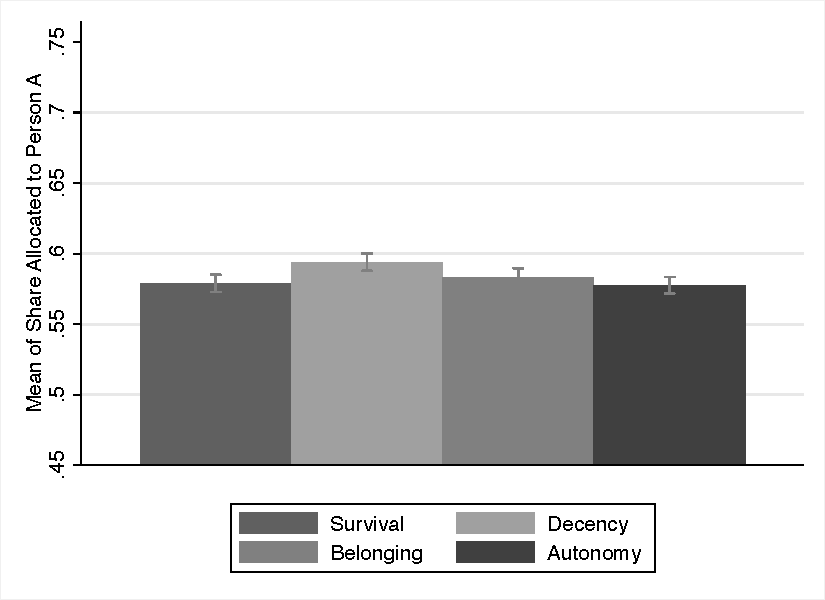
\includegraphics[width=25em]{figures/figure_1.pdf}
   \caption{Bar charts of mean share allocated to Person A per need treatment with 95\% confidence intervals}
   \label{fig:figure_1}
\end{figure}

The data reveals that the share allocated to Person A differs significantly from an equal share of 0.5 in each of our treatments, as $t$ tests show (Survival: $\text{mean}=0.579$, $\text{95\% CI}=[0.573,0.585]$, $p\le0.001$; Decency: $\text{mean}=0.594$, $\text{95\% CI}=[0.588,0.600]$, $p\le0.001$; Belonging: $\text{mean}=0.583$, $\text{95\% CI}=[0.577,0.590]$, $p\le0.001$; Autonomy: $\text{mean}=0.578$, $\text{95\% CI}=[0.572,0.584]$, $p\le0.001$; one-sample $t$ tests, mean tested against 0.5).\footnote{Data is available at \url{https://github.com/alephmembeth/need-deeds/}.}

The influence of the need share also becomes apparent if we take a look at the single cases we presented to our subjects.
Here, the need share of Person A was designed to vary from 0.5 to 0.9.
Clearly, this influences the mean share allocated to Person A per case, as Figure \ref{fig:figure_2} shows.
The mean share allocated to Person A increases from case 1 to 5, correlating with the ascending need share of Person A that rises from 0.5 in case 1 to 0.9 in case 5.
This is further supported by the regression analyses reported in Table \ref{tab:regressions} below.

\begin{figure}[ht]
   \centering
   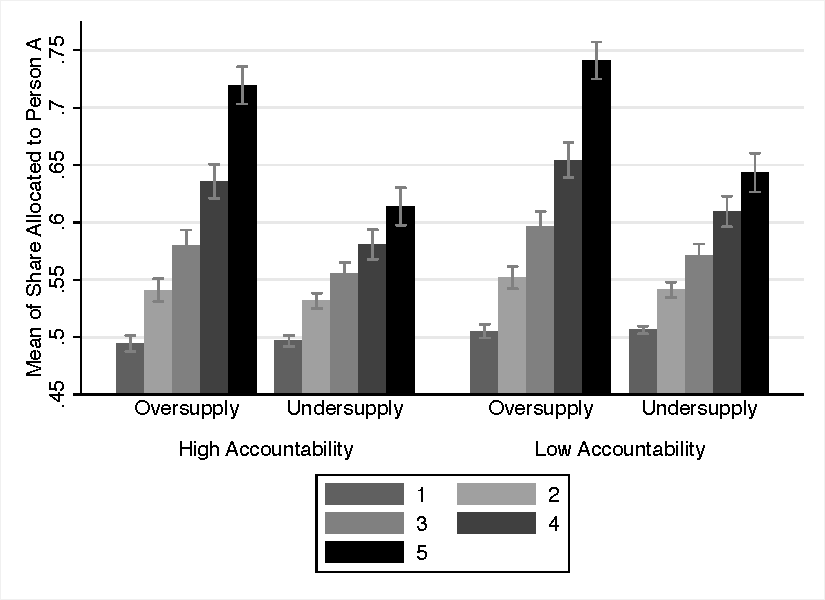
\includegraphics[width=25em]{figures/figure_2.pdf}
   \caption{Bar charts of mean share allocated to Person A per case with 95\% confidence intervals by accountability frame and supply scenario}
   \label{fig:figure_2}
\end{figure}

For further analysis, we can break down the data for the different supply scenarios that were introduced.
Accordingly, Figure \ref{fig:figure_3} shows bar charts of the share our subjects allocated to Person A in the undersupply and oversupply scenario by need treatment.

\begin{figure}[ht]
   \centering
   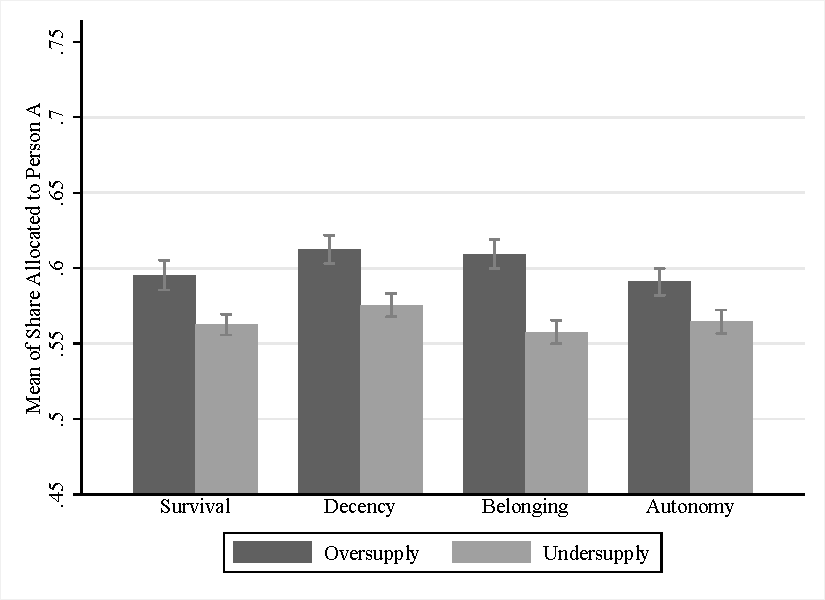
\includegraphics[width=25em]{figures/figure_3.pdf}
   \caption{Bar charts of mean share allocated to Person A in each supply scenario per need treatment with 95\% confidence intervals}
   \label{fig:figure_3}
\end{figure}

Here, $t$ tests indicate that the supply scenario has a highly significant effect on the share subjects allocate to Person A in all treatments.
In general, the mean allocated to Person A is higher in the oversupply scenario than in the undersupply scenario (Survival: $\text{mean difference}=0.033$, $\text{95\% CI}=[0.023,0.043]$, $p\le0.001$; Decency: $\text{mean difference}=0.037$, $\text{95\% CI}=[0.029,0.045]$, $p\le0.001$; Belonging: $\text{mean difference}=0.051$, $\text{95\% CI}=[0.042,0.061]$, $p\le0.001$; Autonomy: $\text{mean difference}=0.026$, $\text{95\% CI}=[0.018,0.035]$, $p\le0.001$; paired-sample two-tailed $t$ test).\footnote{The effect's significance does not change if we test separately for the two accountability frames; Survival, high (low) accountability: $\text{mean difference}=0.035$ ($0.030$), $\text{95\% CI}=[0.021,0.049]$ ($[0.017,0.044]$), $p\le0.001$ ($\le0.001$); Decency, high (low) accountability: $\text{mean difference}=0.039$ ($0.035$), $\text{95\% CI}=[0.027,0.051]$ ($[0.024,0.046]$), $p\le0.001$ ($\le0.001$); Belonging, high (low) accountability: $\text{mean difference}=0.050$ ($0.053$), $\text{95\% CI}=[0.036,0.064]$ ($[0.039,0.067]$), $p\le0.001$ ($\le0.001$); Autonomy, high (low) accountability: $\text{mean difference}=0.030$ ($0.023$), $\text{95\% CI}=[0.018,0.042]$ ($[0.011,0.035]$), $p\le0.001$ ($\le0.001$); paired-sample two-tailed $t$ tests.}

In addition, we suspected an influence of the accountability frame.
Here, Figure \ref{fig:figure_4} shows bar charts of the share our subjects allocated to Person A in the low and high accountability frame by need treatment.

\begin{figure}[ht]
   \centering
   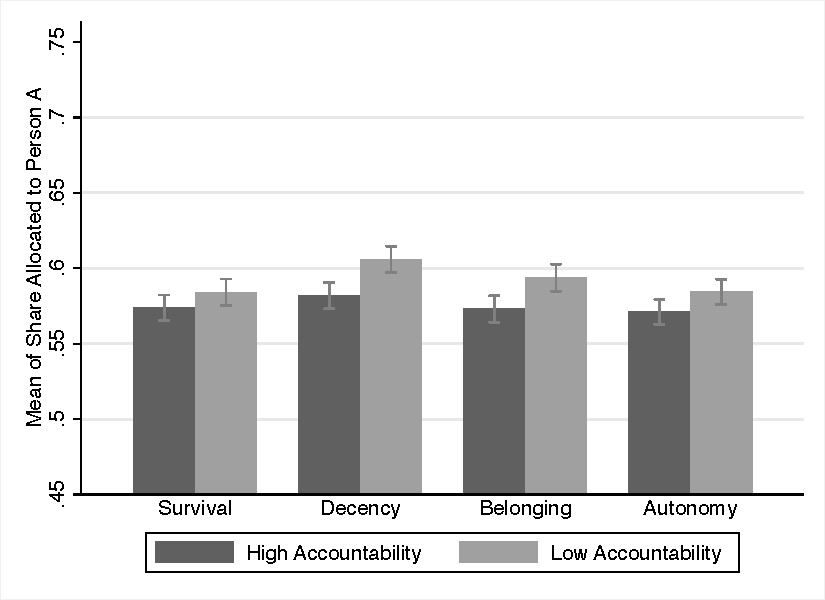
\includegraphics[width=25em]{figures/figure_4.pdf}
   \caption{Bar charts of mean share allocated to Person A in each accountability frame per need treatment with 95\% confidence intervals}
   \label{fig:figure_4}
\end{figure}

Again, we find highly significant effects in all treatments.
In each treatment, the mean allocated to Person A is lower in the high accountability frame than in the low accountability frame (Survival: $\text{mean difference}=-0.010$, $\text{95\% CI}=[-0.016,-0.004]$, $p\le0.001$; Decency: $\text{mean difference}=-0.024$, $\text{95\% CI}=[-0.030,-0.018]$, $p\le0.001$; Belonging: $\text{mean difference}=-0.021$, $\text{95\% CI}=[-0.028,-0.014]$, $p\le0.001$; Autonomy: $\text{mean difference}=-0.013$, $\text{95\% CI}=[-0.020,-0.007]$, $p\le0.001$; paired-sample two-tailed $t$ tests).\footnote{If we test separately for the two supply scenarios, the effect's significance changes for the survival need treatment in the oversupply ($p\le0.1$) and undersupply scenario ($p\le0.01$) as well as for the autonomy need treatment in the oversupply scenario ($p\le0.1$); Survival, oversupply (undersupply): $\text{mean difference}=-0.008$ ($-0.013$), $\text{95\% CI}=[-0.017,0.000]$ ($[-0.020,-0.005]$), $p\le0.1$ ($\le0.01$); Decency, oversupply (undersupply): $\text{mean difference}=-0.022$ ($-0.026$), $\text{95\% CI}=[-0.031,-0.013]$ ($[-0.034,-0.018]$), $p\le0.001$ ($\le0.001$); Belonging, oversupply (undersupply): $\text{mean difference}=-0.022$ ($-0.019$), $\text{95\% CI}=[-0.032,-0.013]$ ($[-0.029,-0.009]$), $p\le0.001$ ($\le0.001$); Autonomy, oversupply (undersupply): $\text{mean difference}=-0.010$ ($-0.017$), $\text{95\% CI}=[-0.018,-0.001]$ ($[-0.027,-0.007]$), $p\le0.1$ ($\le0.001$); paired-sample two-tailed $t$ tests.}
The lower share Person A gets in the high accountability frame is still significantly different from an equal share of 0.5.
So even when they are accountable, subjects acknowledge the hypothetical person's need (Survival, high accountability: $\text{mean}=0.574$, $\text{95\% CI}=[0.565,0.582]$, $p\le0.001$; Decency, high accountability: $\text{mean}=0.582$, $\text{95\% CI}=[0.573,0.591]$, $p\le0.001$; Belonging, high accountability: $\text{mean}=0.573$, $\text{95\% CI}=[0.564,0.582]$, $p\le0.001$; Autonomy, high accountability: $\text{mean}=0.571$, $\text{95\% CI}=[0.563,0.579]$, $p\le0.001$; one-sample $t$ tests, mean tested against 0.5).

Furthermore, we wanted to know whether the different kinds of needs influence the share of logs distributed to Person A.
As Figures \ref{fig:figure_1} to \ref{fig:figure_4} already indicated, this does not seem to be the case, which is further confirmed by the regressions reported in Table \ref{tab:regressions}.

Here, Model (1) is limited to dummy variables for the need treatments, with the survival need treatment as benchmark category.
Model (2) further includes Person A's need share ($0.5,0.6,0.7,0.8,0.9$), the accountability frame ($0=\text{low accountability}$, $1=\text{high accountability}$), and the supply scenario ($0=\text{undersupply}$, $1=\text{oversupply}$).
Lastly, Model (3) adds control variables and Model (4) adds interaction terms (reported in Table \ref{tab:regressions_covariates} in the Appendix).

\begin{table}[ht]
	\centering
	\caption{Regression results (rounded)}\label{tab:regressions}
	\begin{tabular}{ld{3.4}d{3.4}d{3.4}d{3.4}}\\[0.5ex]\hline
		                      & \multicolumn{1}{c}{(1)}         & \multicolumn{1}{c}{(2)}         & \multicolumn{1}{c}{(3)}          & \multicolumn{1}{c}{(4)}          \\\hline\hline
		Need Treatment        &                                 &                                 &                                  &                                  \\
		$\{0=Survival\}$      &                                 &                                 &                                  &                                  \\
		Decency               &  0.015                          &   0.015                         &   0.014                          &   0.019                          \\
		                      & (0.010)                         &  (0.010)                        &  (0.010)                         &  (0.011)                         \\
		Belonging             &  0.004                          &   0.004                         &   0.003                          &  -0.0009                         \\
		                      & (0.010)                         &  (0.010)                        &  (0.010)                         &  (0.012)                         \\
		Autonomy              & -0.001                          &  -0.001                         &  -0.002                          &  -0.003                          \\
		                      & (0.010)                         &  (0.010)                        &  (0.010)                         &  (0.011)                         \\
		A's Need Share        &                                 &   0.436^{***}                   &   0.436^{***}                    &   0.436^{***}                    \\
		$\{[0.5, 0.9]\}$      &                                 &  (0.016)                        &  (0.016)                         &  (0.016)                         \\
		Accountability Frame  &                                 &  -0.017^{***}                   &  -0.017^{***}                    &  -0.010^{**}                     \\
		$\{0=Low, 1=High\}$   &                                 &  (0.003)                        &  (0.003)                         &  (0.004)                         \\
		Supply Scenario       &                                 &   0.037^{***}                   &   0.037^{***}                    &   0.033^{***}                    \\
		$\{0=Under, 1=Over\}$ &                                 &  (0.005)                        &  (0.005)                         &  (0.011)                         \\
		Constant              &  0.579^{***}                    &   0.264^{***}                   &   0.266^{***}                    &   0.265^{***}                    \\
		                      & (0.007)                         &  (0.011)                        &  (0.016)                         &  (0.016)                         \\\hline
		Control Variables     & \multicolumn{1}{c}{\text{No}}   & \multicolumn{1}{c}{\text{No}}   & \multicolumn{1}{c}{\text{Yes}}   & \multicolumn{1}{c}{\text{Yes}}   \\
		$\chi^2$              &  3.090                          & 816.370^{***}                   & 833.810^{***}                    & 841.730^{***}                    \\
		Pseudo-$R^2$ (L1)     &  0.002                          &   0.221                         &   0.230                          &   0.231                          \\
		Pseudo-$R^2$ (L2)     &  0.008                          &   0.008                         &   0.041                          &   0.041                          \\\hline
		\multicolumn{5}{p{11.5cm}}{\footnotesize \textit{Mixed-effects linear regression with robust standard errors. Endogenous variable: share of logs distributed to Person A. First row: coefficients. Second row: standard errors in parentheses. Control variables and interaction terms are reported in Table \ref{tab:regressions_covariates} in the Appendix. Significance levels: * $p \le 0.1$, ** $p \le 0.05$, *** $p \le 0.01$.}}
	\end{tabular}
\end{table}

Model (1) shows that none of the treatment dummies is significant.
Whether Person A is described as needing the wood to fulfil their survival, decency, belonging, or autonomy needs does not influence the share of logs they receive.
However, Model (2) shows that Person A's need share, the accountability frame, and the supply scenario all have a significant impact on their share of logs (estimated slope coefficients: $\text{need share}=0.436$, $\text{95\% CI}=[0.410,0.462]$, $p\le0.001$; $\text{supply scenario}=0.037$, $\text{95\% CI}=[0.029,0.045]$, $p\le0.001$; $\text{accountability frame}=-0.017$, $\text{95\% CI}=[-0.022,-0.012]$, $p\le0.001$).
With each percentage point more of the total need, an additional share of 0.436 percentage points is assigned to Person A.
Moreover, Person A receives additional 3.7 percentage points in the oversupply scenario.
If Person A is accountable for their situation, though, they lose 1.7 percentage points.
Model (3) indicates that all need treatments remain insignificant while the need share, accountability frame, and supply scenario remain highly significant when control variables are included.
Finally, Model (4) shows that all interaction terms are insignificant, except for one.\footnote{To further evaluate if the inclusion of interaction terms positively impacts the quality of Model (4), we ran four additional regressions and performed comparison tests.
Using the same endogenous variable, a first additional model -- Model (5) in Table \ref{tab:regressions_models} -- contains only need treatment and accountability frame without interaction terms, while a second additional model -- Model (6) in Table \ref{tab:regressions_models} -- contains interaction terms for need treatment and accountability frame.
Similarly, a third additional model -- Model (7) in Table \ref{tab:regressions_models} -- contains need treatment and supply scenario without interaction terms, while a fourth additional model -- Model (8) in Table \ref{tab:regressions_models} -- contains interaction terms for need treatment and supply scenario.
Performing two Likelihood Ratio (LR) tests for determining if the interaction terms improve the model's fit, we obtained a $p$ value of 0.249 for Models (5) and (6) as well as a $p$ value of 0.009 for Models (7) and (8), indicating that -- in case of Models (5) and (6) -- the interaction terms do not contribute significantly to a better fit

However, since we are using robust standard errors in our regressions, a LR test must be performed cautiously, and its interpretability is severely limited.
Therefore, we also obtained the Akaike Information Criterion (AIC) and the Bayesian Information Criterion (BIC) for our four additional models, which both serve as metrics for model selection, with a lower value indicating a better fit of the model in question.
Here, Model (5) exhibits slightly lower values ($\text{AIC}=-10224.08$, $\text{BIC}=-10175.17$) than Model (6) ($\text{AIC}=-10222.2$, $\text{BIC}=-10152.33$), while Model (7) ($\text{AIC}=-10370.35$, $\text{BIC}=-10321.44$) in comparison with Model (8) ($\text{AIC}=-10376.01$, $\text{BIC}=-10306.14$) does not.}
All models include a Pseudo-$R^2$ measure as specified by \cite{snijders_modeled_1994} for both the individual level (L1) and the group level (L2), i.e., between the four treatment groups.

Given this between-subjects data, one might be inclined to assume that people do not think that different kinds of needs should lead to different allocations, hence that they all are more or less equally important.
This conclusion might be a bit hasty, though.
While every subject was only introduced to one single kind of need for the main task, we implemented a questionnaire at the end of our study in which we asked subjects to evaluate the importance of all four kinds of needs simultaneously.\footnote{For the following analysis, 15 subjects were excluded because they had one or more missing values for their evaluations of the four kinds of needs.}
Figure \ref{fig:kind_of_need_evaluation_bar} shows the mean importance subjects ascribed to the four kinds of needs in this task.
Each kind of need was rated from 1 (``not important at all'') to 7 (``very important'').

\begin{figure}[ht]
   \centering
   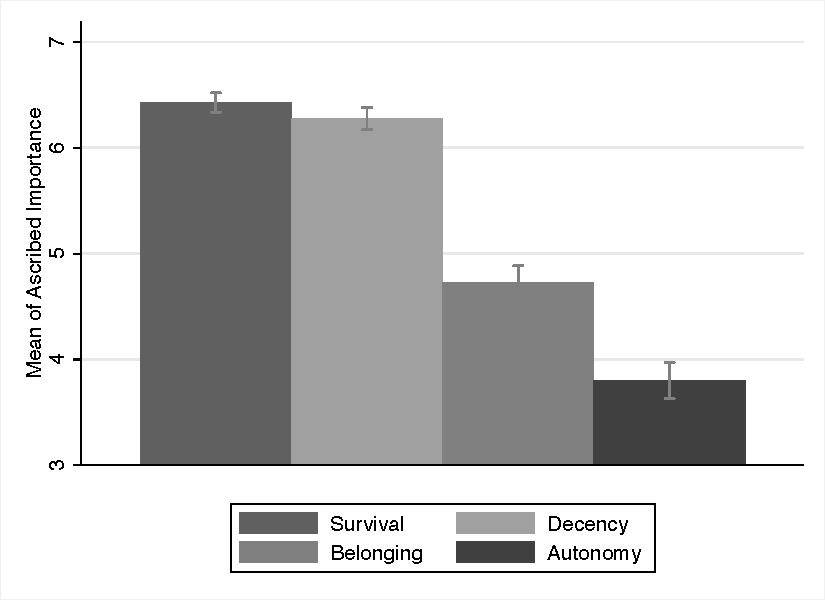
\includegraphics[width=25em]{figures/figure_5.pdf}
   \caption{Bar charts of importance ascribed to each kind of need with 95\% confidence intervals}
   \label{fig:kind_of_need_evaluation_bar}
\end{figure}

As can be seen here, most subjects rated the importance of survival need and decency need as very high (Survival: $\text{mean}=6.434$, $\text{std. dev.}=0.906$; Decency: $\text{mean}=6.275$, $\text{std. dev.}=1.037$).
The importance of belonging need and autonomy need, however, is clearly evaluated lower (Belonging: $\text{mean}=4.701$, $\text{std. dev.}=1.584$; Autonomy: $\text{mean}=3.783$, $\text{std. dev.}=1.706$).
Accordingly, a one-way repeated measures ANOVA reveals a significant effect of the kind of need on the evaluation of its importance ($F(3,1572)=351.090$, $p\le0.001$), allowing us to reject the null hypothesis that -- in this task -- the mean evaluation for all four kinds of needs is equal.

As Table \ref{tab:evaluations} further shows, pairwise comparisons of all kinds of needs -- except for survival versus decency -- are significant at the $p\le0.001$ level.
Hence, we can conclude that -- except for survival versus decency -- subjects ascribe distinctly different evaluations of importance to the different kinds of needs.

\begin{table}[ht]
   \centering
   \caption{Mean importance ascribed to kinds of needs and differences between them}\label{tab:evaluations}
   \begin{tabular}{rd{2.4}d{2.4}d{2.4}d{2.4}}\hline
                  & \multicolumn{1}{c}{Survival}   & \multicolumn{1}{c}{Decency}   & \multicolumn{1}{c}{Belonging}   & \multicolumn{1}{c}{Autonomy}   \\\hline
      Mean        &  6.429                         &  6.275                        &  4.730                          & 3.802                          \\
      Std. Dev.   &  0.910                         &  1.044                        &  1.554                          & 1.702                          \\\hline\hline
      Decency     & -0.153                         &                               &                                 &                                \\
      Belonging   & -1.699^{***}                   & -1.545^{***}                  &                                 &                                \\
      Autonomy    & -2.626^{***}                   & -2.473^{***}                  & -0.927^{***}                    &                                \\\hline
      \multicolumn{5}{p{9.5cm}}{\footnotesize{\textit{Upper panel: mean of ascribed importance, standard deviation, and number of observations. Lower panel: mean differences. $n=385$. Significance levels: * $p \le 0.1$, ** $p \le 0.05$, *** $p \le 0.001$, Bonferroni adjusted.}}}
   \end{tabular}
\end{table}

To summarize, our analysis has shown that there is no between-subjects effect of the different need treatments; subjects do evaluate the kinds of needs differently, though, when presented with all of them on a within-subjects level.
Furthermore, we have shown that subjects' distribution decisions are influenced by the neediness of a person, which is moderated by their accountability and the general resource availability.


\section{Conclusion}\label{sec:conclusion}
This brief chapter presented a follow-up study to \cite{bauer_need_2022} in which we tested for the effects of need, accountability, and resource availability on third-party distribution decisions as well as for the possible effects of different kinds of needs.

We did not find significant differences in distribution decisions between the four need treatments.
This, we assume, is the case because the differences in the rather long vignette texts were relatively small.
Presumably, this was not enough to make the different kinds of needs and their implications salient.
Our questionnaire at the study's end gives some support to this assumption.
Here, subjects had to evaluate the importance of the four kinds of needs simultaneously on a scale from ``not important at all'' to ``very important''.
A clear majority of subjects rated the importance of the needs for survival and decency as very high.
The importance of the needs for belonging and autonomy, on the other hand, was evaluated distinctly lower.
We take this as an indication that further studies are needed to test the possible influence of different kinds of needs on distribution decisions.

Moreover, we found that subjects tend to distribute the firewood unequally between the two hypothetical persons, even though both have contributed equally to the total amount available for redistribution.
This is the case in all four need treatments.
In each of them, the (mean) share of the total amount distributed to the needier person is significantly higher than an equal share of 0.5.
Hence, in the distribution task, all kinds of needs mattered to our subjects, and none of them was perceived as superfluous or irrelevant with regard to a just distribution.
As our regression revealed, this effect is not only influenced by the accountability frame and by Person A's need share (as we have already seen in \citealt{bauer_need_2022}) but clearly also by the supply scenario.
In sum, the mean subjects allotted to the person experiencing the higher need was significantly lower when this person was accountable.
Nonetheless, even when accountable, this person received a higher share of logs than their initial contribution would suggest.
This share was even bigger when there was a surplus of resources.

Consequently, our findings bear some noteworthy implications.
First, it is important to note that we successfully replicated key findings from \cite{bauer_need_2022}, even though we slightly modified the vignette, changed the parametrization, and implemented the accountability variation within subjects instead of between subjects.
This gives even more weight to the data implicating that laypeople consider the factors of need and accountability when thinking about just distributions.
Given our study's new data, we can now confidently add that they also take resource availability into consideration.
Unfortunately, our data is less clear when it comes to the role different kinds of needs may play.
Here, subjects treated each kind of need as similarly important in our between-subjects treatments.
When they were asked to directly compare the kinds of needs, though, a pattern emerged that shows that needs are perceived as differently important.
Clearly, further research is needed in this regard.


\clearpage
\bibliographystyle{elsarticle-harv}
\bibliography{references}


\clearpage
\appendix
\section{Instructions of the Study}\label{sec:app_instructions}
\subsection*{Welcome Screen}
In this survey, we are interested in your personal opinion and judgment.
Therefore, there are no correct or incorrect answers in this study.
Participation in this study is voluntary, you can cancel it at any time.

If you work intently, it will probably take you about 30 minutes.
It is important that you complete the study without interruption and without closing your browser.
If you cannot avoid closing your browser, you can continue the study by clicking the Mingle link anew.

During the course of the study, we will ask you a total of three attention questions.
With these we want to make sure that you read and understand the instructions correctly.
If you answer more than one of these questions incorrectly, you will automatically be excluded from the study.

We will analyse your answers together with the answers of all other participants in this study.
All data will be stored in an anonymous format so that no participant can be identified.
The results of the study will be published.
They may influence future research and may be used to inform policymakers.

Thank you for participating!


\subsection*{Introduction}
Your task is to distribute logs of wood.

We will present to you a number of different scenarios and ask you to imagine that they are real.
Please take the time to immerse yourself in the scenarios and come to a personal assessment.

In these scenarios, when moving from screen to screen, text that differs from the previous page is highlighted in blue.
Text that is similar to that in the previous page is not highlighted in blue.

\subsection*{Vignette Text and Variations of the Need Treatments}
\noindent\textit{Note: We randomised the names displayed, denoted as $A$ and $B$ below (``Müller'', ``Schmidt'', ``Schneider'', ``Fischer'', ``Weber'', ``Meyer'', based on frequent German surnames), as well as the orderings of the table (with the needier person in the upper or lower row and the information of need and wood chopped interchanged).}\vspace{2ex}

\noindent\textbf{Opening:} Please imagine two people, $A$ and $B$.
$A$ and $B$ do not know each other.
Both need wood.
The community of $A$ and $B$  allows them to cut down trees in the community forest for a certain period of time.
$A$ and $B$ have little money and therefore have no other means to get wood.\vspace{2ex}

\noindent\textbf{Survival:} $A$ and $B$ need the wood to make sure they survive the upcoming winter since they heat their huts exclusively with wood.
To do so, $A$ needs $r$ logs of wood and $B$ needs $s$ logs of wood.
[Case 5: To do so, both $A$ and $B$ need $r$ logs of wood.]

If they get less than they need, their huts become so cold that they are likely to get life-threateningly ill.
The less wood they get, the higher the probability that they will get life-threateningly ill.
If $A$ and $B$ get more wood than they need, they can store it for subsequent winters.\vspace{2ex}

\noindent\textbf{Decency:} $A$ and $B$ need the wood to not feel unreasonably cold in the upcoming winter since they heat their huts exclusively with wood.
To do so, $A$ needs $r$ logs of wood and $B$ needs $s$ logs of wood.
[Case 5: To do so, both $A$ and $B$ need $r$ logs of wood.]

If they get less than they need, their huts become unreasonably cold.
The less wood they get, the more often it will get unreasonably cold.
Their community agrees that one cannot live a decent life if one has to feel unreasonably cold.
If $A$ and $B$ get more wood than they need, they can store it for subsequent winters.\vspace{2ex}

\noindent\textbf{Belonging:} $A$ and $B$ need the wood to be able to take part in the social life regularly during winter since it is common practice to meet in the community centre and that everyone brings wood to heat it.
To do so, $A$ needs $r$ logs of wood and $B$ needs $s$ logs of wood.
[Case 5: To do so, both $A$ and $B$ need $r$ logs of wood.]

If they get less than they need, they will not be able to attend community get-togethers regularly.
The less wood they get, the less often they will be able to attend community get-togethers.
If $A$ and $B$ get more wood than they need, they can store it for subsequent winters.\vspace{2ex}

\noindent\textbf{Autonomy:} $A$ and $B$ need the wood to be able to use their ateliers since they heat their ateliers exclusively with wood.
Here, they spend their leisure time to create art.
To do so, $A$ needs $r$ logs of wood and $B$ needs $s$ logs of wood.
[Case 5: To do so, both $A$ and $B$ need $r$ logs of wood.]

If they get less than they need, they will not be able to use their ateliers regularly.
The less wood they get, the less often they will be able to use their ateliers.
If $A$ and $B$ get more wood than they need, they can store it for subsequent winters.\vspace{2ex}

\noindent\textbf{Low responsibility:} $A$ suffers from a congenital metabolic disease.
Because of this disease, $A$ needs a higher room temperature than $B$.
This is why $A$ needs more wood than $B$.
[Case 5: Nonetheless, $A$ needs the same amount of wood as $B$.]\vspace{2ex}

\noindent\textbf{High responsibility:}
$A$ continued to smoke heavily against the advice of their doctor and therefrom suffers from a metabolic disease.
Because of this disease, $A$ needs a higher room temperature than $B$.
This is why $A$ needs more wood than $B$.
[Case 5: Nonetheless, $A$ needs the same amount of wood as $B$.]\vspace{2ex}

\noindent\textbf{Closing:}
$A$ and $B$ have chopped $p$ logs of wood each.
Taken together, both have chopped $q$ logs of wood.
In the table, you can see how much wood the persons have chopped and how much wood they need.
In the free fields, please distribute the wood between the two persons in the way that you think is most just.
Please distribute all $q$ logs.\vspace{2ex}

There are $n$ logs left.

\begin{table}[ht]
   \centering
   \begin{tabular}{cccc}\hline
      Person   & has chopped   & needs   & should receive   \\\hline\hline
      $A$      & $p$           & $r$     & $u$              \\
      $B$      & $p$           & $s$     & $v$              \\\hline
      Total    & $q$           & $t$     & $w$              \\\hline
      \multicolumn{4}{p{7.5cm}}{\footnotesize \textit{$p$, $q=p*2$, $r$, $s$, and $t=r+s$ were provided as parameters of our study, while participants were asked to provide input for $u$ and $v$; $n$ and $w=u+v$ were automatically calculated while they did so.}}
   \end{tabular}
\end{table}


\clearpage
\section{Additional Questions}\label{sec:app_questions}

\subsubsection*{Control Questions}
\noindent\textit{Note: Options for Questions 2 and 3 were displayed in randomized order.}\vspace{1ex}

\noindent\textbf{Question 1:} Please describe how often you reflect on justice issues in your daily life and what this means to you.

We ask this question to ensure that the tasks are read carefully.
If you are reading this, please enter the number 42 in the field below instead of an answer to the question itself.

Have you ever dealt with justice issues?\vspace{1ex}

\noindent\textbf{Question 2:} Which statements apply to this study?
Multiple answers are possible.
\begin{itemize}
   \item[$\square$] Farmers work a rye field.
   \item[$\square$] Farmers work a sunflower field.
   \item[$\square$] Farmers work a wheat field.
   \item[$\square$] Wood is needed to build a house.
   \item[$\square$] Wood is needed to heat in winter.
   \item[$\square$] Water is needed to run a mill.
   \item[$\square$] Water is needed to drink.
\end{itemize}\vspace{1ex}

\noindent\textbf{Question 3:} What was the largest quantity of logs to be distributed in the previous scenarios?
\begin{itemize}
   \item[$\square$] 500
   \item[$\square$] 1000
   \item[$\square$] 1200
   \item[$\square$] 1800
   \item[$\square$] 2500
   \item[$\square$] 3000
   \item[$\square$] 5000
\end{itemize}

\subsubsection*{Support for Different Distribution Principles}
\noindent\textit{Note: Items were displayed in a randomized order. Each scale included a value for ``no answer/I don't know''.}\vspace{1ex}

\noindent How important have the following considerations been to your distributions?
Please give your answers on the scales from 1 (not at all important) to 7 (very important).
\begin{itemize}
   \item Each person should receive as much wood as they need.
   \item Each person should receive the wood they have chopped.
   \item Each person should receive the same amount of wood.
\end{itemize}

\subsubsection*{Locus of Control}
\noindent\textit{Note: Items were displayed in a randomized order. Each scale included a value for ``no answer/I don't know''.}\vspace{1ex}

\noindent Please indicate on the following scales from 1 (not at all) to 7 (very much) how much you agree with the following statements.
\begin{itemize}
   \item I am in control of my life.
   \item If I make an effort, I am going to succeed.
   \item Whether in my private life or at work, my life is largely determined by others.
   \item My plans are often thwarted by fate.
\end{itemize}

\subsubsection*{Political Orientation}
\noindent\textit{Note: The scale included a value for ``no answer/I don't know''.}\vspace{1ex}

\noindent In politics, one speaks of left-wing and right-wing.
How would you generally describe your own political position?
On a scale from 1 (left) to 7 (right), where would you rate yourself?

\subsubsection*{Kinds of Needs}
\noindent\textit{Note: We asked subjects for the importance they ascribe to the kind of need that was presented to them in the main task as part of the need treatment.
On a subsequent page, we asked them to evaluate the importance of the three other kinds of needs.
Answers were given on scales from 1 (not at all important) to 7 (very important).
Each scale included a value for ``no answer/I don't know''}.\vspace{1ex}

\noindent On the previous pages, $A$ and $B$ needed wood to make sure they survive the upcoming winter (to not feel unreasonably cold in the upcoming winter/to be able to take part in the social life regularly during winter/to be able to use their ateliers).
How important do you think it is to meet this need?\vspace{1ex}

\noindent Please indicate how important you consider the following kinds of needs that can be met with the help of firewood.
\begin{itemize}
   \item Heating to make sure to survive the upcoming winter.
   \item Heating to not feel unreasonably cold in the upcoming winter.
   \item Heating to be able to take part in the social life regularly during winter.
   \item Heating to be able to use one's atelier.
\end{itemize}


\clearpage
\section{Additional Tables}\label{sec:app_tables}

\begin{table}[ht]
   \centering
   \caption{Regression results (rounded) for control variables and interaction terms}\label{tab:regressions_covariates}
   \begin{tabular}{ld{2.5}d{2.5}}\\[0.5ex]\hline
                                        & \multicolumn{1}{c}{(3)}   & \multicolumn{1}{c}{(4)}   \\\hline\hline
      Age                               &  0.000                    &  0.000                    \\
      $\{\sharp years\}$                & (0.000)                   & (0.000)                   \\
      Gender                            &  0.003                    &  0.003                    \\
      $\{0=female,1=male\}$             & (0.007)                   & (0.007)                   \\
      Equivalent Household Net Income   &  0.000                    &  0.000                    \\
      $\{euros\}$                       & (0.000)                   & (0.000)                   \\
      Importance Need                   &  0.000                    &  0.000                    \\
      $\{1,\ldots,7\}$                  & (0.000)                   & (0.000)                  \\
      Importance Equity                 & -0.001^{***}              & -0.001^{***}              \\
      $\{1,\ldots,7\}$                  & (0.001)                   & (0.001)                  \\
      Importance Equality               & -0.000                    & -0.000                   \\
      $\{1,\ldots,7\}$                  & (0.000)                   & (0.000)                  \\
      Decency\#High Accountability      &                           & -0.014^{*}                \\
                                        &                           & (0.007)                   \\
      Belonging\#High Accountability    &                           & -0.010                    \\
                                        &                           & (0.008)                   \\
      Autonomy\#High Accountability     &                           & -0.003                    \\
                                        &                           & (0.007)                   \\
      Decency\#Oversupply               &                           &  0.004                    \\
                                        &                           & (0.014)                   \\
      Belonging\#Oversupply             &                           &  0.019                    \\
                                        &                           & (0.015)                   \\
      Autonomy\#Oversupply              &                           & -0.006                    \\
                                        &                           & (0.014)                   \\\hline
      \multicolumn{3}{p{10cm}}{\footnotesize \textit{Results for the control variables of Models (3) and (4) as well as the interaction terms of Model (4) in Table \ref{tab:regressions}. Mixed-effects linear regression with robust standard errors. Endogenous variable: share of logs distributed to Person A. First row: coefficients. Second row: standard errors in parentheses. Significance levels: *~$p\le0.1$, **~$p\le0.05$, ***~$p\le0.01$.}}
   \end{tabular}
\end{table}

\begin{table}[ht]
   \centering
   \caption{Regression results (rounded) for evaluation of interaction terms}\label{tab:regressions_models}
   \begin{tabular}{ld{2.4}d{2.4}d{2.4}d{2.4}}\\[0.5ex]\hline
                                       & \multicolumn{1}{c}{(5)}   & \multicolumn{1}{c}{(6)}   & \multicolumn{1}{c}{(7)}   & \multicolumn{1}{c}{(8)}   \\\hline\hline
      Need Treatment                   &                           &                           &                           &                           \\
      $\{0=Survival\}$                 &                           &                           &                           &                           \\
      Decency                          &  0.015                    &  0.022^{**}               &  0.015                    &  0.013                    \\
                                       & (0.010)                   & (0.011)                   & (0.010)                   & (0.011)                   \\
      Belonging                        &  0.004                    &  0.010                    &  0.004                    & -0.005                    \\
                                       & (0.010)                   & (0.011)                   & (0.010)                   & (0.011)                   \\
      Autonomy                         & -0.001                    & -0.000                    & -0.001                    & -0.002                    \\
                                       & (0.010)                   & (0.011)                   & (0.010)                   & (0.011)                   \\
      Accountability Frame             & -0.017^{***}              & -0.010^{**}               &                           &                           \\
      $\{0=Low, 1=High\}$              & (0.003)                   & (0.004)                   &                           &                           \\
      Decency\#High Accountability     &                           & -0.014                    &                           &                           \\
                                       &                           & (0.007)                   &                           &                           \\
      Belonging\#High Accountability   &                           & -0.010                    &                           &                           \\
                                       &                           & (0.008)                   &                           &                           \\
      Autonomy\#High Accountability    &                           & -0.003                    &                           &                           \\
                                       &                           & (0.007)                   &                           &                           \\
      Supply Scenario                  &                           &                           &  0.037^{***}              &  0.033^{***}              \\
      $\{0=Under, 1=Over\}$            &                           &                           & (0.005)                   & (0.011)                   \\
      Decency\#Oversupply              &                           &                           &                           &  0.004                    \\
                                       &                           &                           &                           & (0.014)                   \\
      Belonging\#Oversupply            &                           &                           &                           &  0.019                    \\
                                       &                           &                           &                           & (0.015)                   \\
      Autonomy\#Oversupply             &                           &                           &                           & -0.006                    \\
                                       &                           &                           &                           & (0.013)                   \\
      Constant                         &  0.588^{***}              &  0.584^{***}              &  0.561^{***}              &  0.563                    \\
                                       & (0.007)                   & (0.008)                   & (0.007)                   & (0.007)                   \\\hline
      $\chi^2$                         & 38.810^{***}              & 40.600^{***}               & 63.660^{***}               & 65.460^{***}            \\
      Pseudo-$R^2$ (L1)                &  0.006                    &  0.006                    &  0.020                    &  0.021                    \\
      Pseudo-$R^2$ (L2)                &  0.008                    &  0.008                    &  0.008                    &  0.008                    \\\hline
      \multicolumn{5}{p{13cm}}{\footnotesize \textit{Results for Models (5) to (8). Mixed-effects linear regression with robust standard errors. Endogenous variable: share of logs distributed to Person A. First row: coefficients. Second row: standard errors in parentheses. Significance levels: *~$p\le0.1$, **~$p\le0.05$, ***~$p\le0.01$.}}
   \end{tabular}
\end{table}

\begin{table}[ht]
   \centering
   \caption{Breakdown of the sample by gender, age, and income}\label{tab:demos}
   \begin{tabular}{rrrrrr}\\[0.5ex]\hline
      \multicolumn{2}{c}{Gender}   & \multicolumn{2}{c}{Age}   & \multicolumn{2}{c}{Income$^a$}   \\\hline
      Group     & Share            & Group     & Share         & Group             & Share        \\\hline\hline
      Female    & 49.75            & $18-29$   & 21.11         & $[0,1500)$        & 16.08        \\
      Male      & 50.00            & $30-39$   & 18.09         & $[1500,2500)$     & 22.86        \\
      Diverse   &  0.25            & $40-49$   & 18.84         & $[2500,3500)$     & 23.12        \\
                &                  & $50-59$   & 23.87         & $[3500,4500)$     & 19.10        \\
                &                  & $60-74$   & 18.09         & $[4500,\infty)$   & 18.84        \\\hline
   \multicolumn{6}{p{9cm}}{\footnotesize{\textit{Share in percent. $n=400$. $^a$Equivalent household net income (interval notation).}}}
   \end{tabular}
\end{table}

\end{document}
